\chapter{Implementacja}

Moduł ekstrakcji podsumowań danych został zaimplementowany zgodnie z przedstawionym wcześniej diagramem klas. W tym rozdziale omówiono narzędzia wykorzystane w trakcie implementacji. Oprócz tego przedstawiono niektóre zastosowane rozwiązania oraz przykład działania.


\section{Narzędzia i środowisko wykonawcze}

Podczas implementacji modułu nie zostały użyte żadne zewnętrzne biblioteki, ani \textit{frameworki} (platformy programistyczne). Korzystano jedynie z biblioteki standardowej (\textit{Java} 1.8) oraz źródeł literaturowych -- np. \cite{java}.

Środowisko wykonawcze z jakiego korzystano to \textit{IntelliJ IDEA (Ultimate Edition)} w~wersji 2018.3.2. Zawiera ono wiele przydatnych narzędzi -- np. \textit{Database} (rysunek \ref{rys:database}), które pozwala podczas działania aplikacji połączyć się z bazą danych w czasie rzeczywistym uruchomić podgląd dowolnej tabeli i dodawać nowe rekordy do bazy. Pozwala to na ręczne zasymulowanie procesu pojawiania się nowych obserwacji w źródłowej bazie danych.

\begin{figure} 
	\centering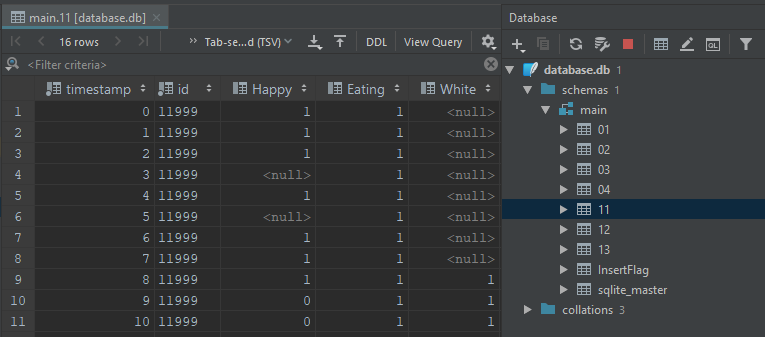
\includegraphics[width=\textwidth]{img/database}
	\caption{Narzędzie \textit{Database} w programie \textit{IntelliJ IDEA}}
	\label{rys:database}
\end{figure}


\section{Rozwiązania programistyczne}

W niniejszym podrozdziale przytoczone zostały wybrane fragmenty kodu, które mają stosunkowo największy wpływ na spełnienie zdefiniowanych uprzednio wymagań.

Pierwszy przykład (przedstawiony w \ref{lis:holon1}) dotyczy aktualizowania holonów wykorzystując \textit{retrospectiveCard}, czyli wspomnianą wcześniej retrospektywną moc zbioru. Jest to liczba całkowita przechowywana w holonie, której wartość mówi o ilości epizodów, z~jakich obliczone zostały podsumowania. \textit{Tao} z kolei przechowuje wartości podsumowań. W~zamieszczonym fragmencie działanie $ tao.getK() * retrospectiveCard $ przywraca ilość faktycznych epizodów, do których można następnie dodać nowe epizody (analogiczne działanie) i obliczyć nowe wartości podsumowań.

\begin{listing}
\begin{minted}{java} 
private void updateTao(double sumPositive, double sumNegative, int groundSetCard) {
	sumPositive = sumPositive * groundSetCard + tao.getK() * retrospectiveCard;
	sumNegative = sumNegative * groundSetCard + tao.getV() * retrospectiveCard;
	retrospectiveCard += groundSetCard;
	tao.setK(sumPositive / retrospectiveCard);
	tao.setV(sumNegative / retrospectiveCard);
}
\end{minted}
	\caption{Aktualizowanie wartości podsumowań holonu prostego} 
	\label{lis:holon1}
\end{listing}

Następny fragment kodu (listing \ref{lis:holon2}) dotyczy przekazywania holonowi do aktualizacji tylko nowych epizodów -- czyli wszystkich które pojawiły się od czasu ostatniej aktualizacji. Wykorzystano w tym celu strumienie, które są nową funkcją w \textit{Java}'ie \textit{1.8} (więcej informacji na ten temat -- \cite{java}).

\begin{listing}
\begin{minted}{java} 
private void updateHolon(Holon holon) {
	Set<BaseProfile> newBaseProfiles = baseProfilesRepository.stream().
		filter(h -> h.getTimestamp() > holon.getTimestamp()).
		collect(Collectors.toCollection(TreeSet::new));
	holon.update(newBaseProfiles, currTimestamp);
}
\end{minted}
	\caption{Przekazywanie nowych epizodów do aktualizacji holonu} 
	\label{lis:holon2}
\end{listing}


\section{Przykład działania agenta}

W tej części przedstawiony zostanie przykład działania agenta z wykorzystaniem scenariuszy, gdyż ten sposób będzie wykorzystany również w kolejnym rozdziale. Dodatkowo jest to rozwiązanie bardzo wygodne i szybkie. Wykorzystuje ono odpowiednio sformatowane pliki CSV (rysunek \ref{rys:scenariusz}). W pliku zawarte są obiekty, obserwacje oraz pytania. Istnieje możliwość zadania innego pytania po każdym rekordzie. Obok podać można oczekiwaną odpowiedź. Wynik przetwarzania tego przykładu przedstawia rysunek \ref{rys:wynik}.

\begin{figure}  
	\centering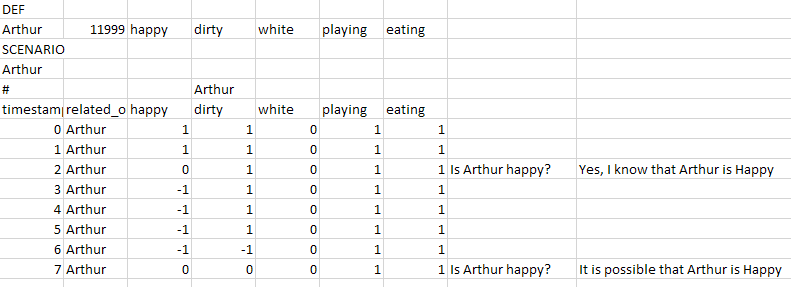
\includegraphics[width=\textwidth]{img/scenariusz}
	\caption{Przykładowy plik CSV scenariusza}
	\label{rys:scenariusz}
\end{figure}

\begin{figure}  
	\centering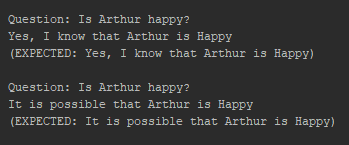
\includegraphics[width=.5\textwidth]{img/wynik}
	\caption{Wynik przetwarzania scenariusza z rysunku \ref{rys:scenariusz}}
	\label{rys:wynik}
\end{figure}








